\chapter{Web Threats} \label{sec:sectionTwo}
\section{What is a Web Threat}

At its most basic definition, a web threat is any malicious attack that uses the Internet as its main method of distribution, meaning the types of web threats is wide and varied.  Web threats can be broken up into two main categories referred to as push or pull.  Pull based threats are attacks that can affect any visitor to the website or service while push based attacks use luring techniques to get a user to fall victim to the attack such as phishing emails.  The main motivation behind these attacks is the pursuit of confidential information and it is becoming increasingly commonplace to hear about large scale data breaches.  While it is difficult to track all of the monetary gain from these activities due to their underground nature, there are some recorded instances of extortion upwards of millions of dollars from even large businesses.  As the number of users and the complexity of the devices attached to these networks increases so to it does the exploitability.  Common web attacks can range from simple phishing emails, to malicious email attachments to malicious code injection directly into a vulnerable website and is a very serious problem.

Attackers will vary their methods and tools often which creates a situation where the limitless number of possible attacks always keeps the attacker a step ahead of the prevention systems.  This leads to the conclusion that conventional approaches grand-fathered in from other security sectors such as virus scanning are not adequate enough for web threat detection.  There are two important reasons for this: first off the attacks vary in their approaches and transportation techniques so widely that collecting samples to produce signatures for detection is not feasible.  The second reason is unlike conventional viruses which attempt to spread as fast as possible, web attacks instead try their best to go under the radar and avoid detection.  In addition, web servers are required to be publically open to the world unlike traditional desktop computers which typically have all their ports closed, by accepting information from unknown parties by default many problems are created.  Therefore, modern solutions employ a much more layered approach using conventional detection methods along with reputation systems, feedback loops, and other systems to increase the overall security (Section \ref{sec:sectionThree}) \cite{trendMicro}.

\begin{figure}
	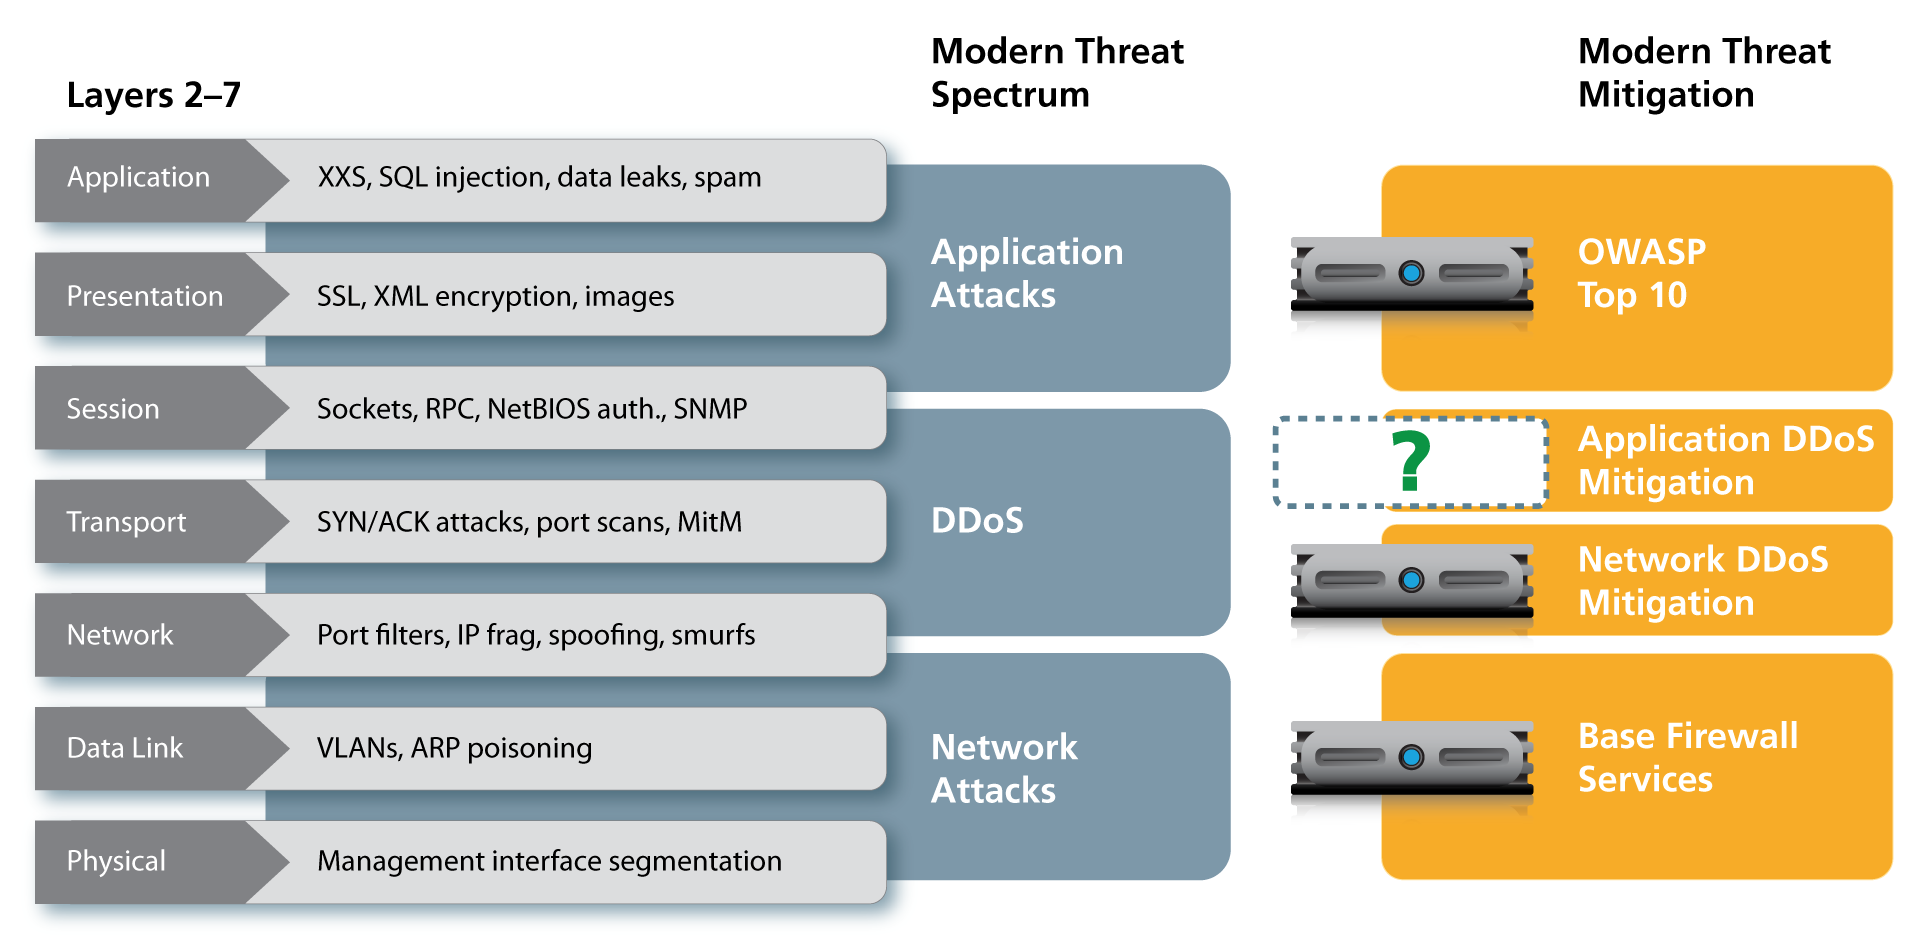
\includegraphics[width=450px]{./assets/img/osithreats.png}
	\caption{Possible threats at each OSI model layer and possible mitigation techniques. {\cite{f5whitepaper}} }
	\label{fig:osithreats}
\end{figure}

Web threats can target any layer of the OSI model in order to exploit different weaknesses or perform different types of attacks for various reasons (Figure \ref{fig:osithreats}).  Application attacks, which this research is focusing on, occur on the Application, Presentation, and partially, the Session layers.  Prevention of the OWASP Top10 security flaws can mitigate several of these attacks, but the keyword is mitigation, there is always the possibility for a new attack variant to slip past existing safeguards.

Attackers will always prefer the most vulnerable target, the weakest link, and there is nothing more vulnerable than the public-facing application itself.  Studies have found many of the existing techniques for handling these application layer attacks suffer from one or more of the following techniques \cite{aSurveyOnWeb}:

\begin{itemize}
	\setstretch{1.0}
	\item Inherent limitations
	\item Incomplete implementations
	\item Complex frameworks
	\item Runtime overheads
	\item Intensive manual work requirements
	\item False positives and false negatives
\end{itemize}

This means that despite the fact that these attacks are commonly considered easy to mitigate, the existing solutions are not completely adequate in some aspect for defending against some of the most common web attacks.  Exploration of new methods of detection and prevention, as well as improvement of older conventional methods is necessary in order to solve these problems.

\section{SQL Injection}\label{sec:sqliExplanation}
Structured Query Language or SQL for short is the most dominant language for interacting with relational databases in recent years.  A SQL injection is an attack where through various means arbitrary unauthorized SQL code is ran on the database.  As the prime motivator for these attacks that was discussed was gathering confidential data, this is a very powerful way of acquiring said information \cite{aSurveyOnWeb}.  There are four common methods of injecting SQL commands into an application:

\begin{itemize}
	\setstretch{1.0}
	\item Injection through user input
	\item Injection through cookies
	\item Injection through server variables
	\item Second-order injections
\end{itemize}

Injection through user input is the simplest of the methods, the malicious user simply enters the arbitrary SQL code into any field that has some form of interaction with the database.  Injection through cookies involves exploiting applications that read from the cookie's fields to restore the user's state by modifying this information to contain SQL code.   The application will then read this modified information upon returning to the website.  Server variables (such as PHP session variables, or other environment variables) operate similarly to cookies in applications which as a result are exploitable in a similar fashion.    Lastly, second-order injections are some of the hardest SQL injection to detect because they involve an attack that occurs at a later point after the initial exploit is entered \cite{aClassificationOfSQL}.

The impact and purpose of SQL injections can also be broken down into four main categories.  First, \textbf{confidentiality} is lost, databases that hold sensitive information which may be financial or identifiable is compromised and should now be considered public knowledge.  Secondly, in addition to the data being potentially leaked publically, it now has also lost its \textbf{integrity} as the malicious user can make any modification he/she wants.  \textbf{Authentication} and \textbf{authorization} of the application is also broken, it is now possible to log in as any user with any access level, removing the need and purpose for passwords and safeguards.

However, there is a threat of much more dangerous activities than just simply retrieving the information contained within a database through the use of SQL injections.  For example, previous wide-scale botnet attacks have used SQL injections mimicking as Google queries in order to facilitate malicious drive-by-download malware attacks on websites \cite{aSurveyOnWeb}.

\subsection{SQL Injection Types}\label{sec:sqliTypes}

Often times a combination of several injection types make up a single SQL injection attack, and so the distinctions are not necessarily absolute, but the techniques can be broken down and classified under the six following categories:

\textbf{Tautology} attacks by their design, attempt to bypass authentication, identify injectable parameters or extract data; often by using conditional SQL statements to evaluate to true within the WHERE portion of the query.  This will result in the query evaluating to true for every single row in a given table often returning all of the rows depending on how the application as well as the injection query is designed. For example, the '1=1' portion of the following query will always evaluate to true, and the remainder of the query is removed using the SQL comment character '--' (Snippet \ref{snippet:tautology}).

\begin{codesnippet}
	\vspace{0.25in}
	\noindent
	\code{SELECT accounts FROM users WHERE login=’’ or 1=1 -- AND pass=’’ AND pin=}
	\captionof{snippet}{Example tautology SQLi attack \cite{aClassificationOfSQL}}
	\label{snippet:tautology}
	\vspace{0.25in}
\end{codesnippet}

A \textbf{malformed} or invalid query are performed to gather information about the underlying database or applications structure in order to design targeted queries.  This is due to the common mistake of having overly descriptive errors that reveal information that can be very useful to an attacker. This information can reveal information ranging from the DBMS used to the names of columns or tables.  The following example forces a conversion error (Snippet \ref{snippet:malformed}).

\begin{codesnippet}
	\vspace{0.25in}
	\noindent
	\code{SELECT accounts FROM users WHERE login=’’ AND pass=’’ AND pin= convert \\
(int,(select top 1 name from sysobjects where xtype=’u’))}
	\captionof{snippet}{Example malformed SQLi attack \cite{aClassificationOfSQL}}
	\label{snippet:malformed}
	\vspace{0.25in}
\end{codesnippet}

A third type of SQL injection exploits the \textbf{union} keyword which is used to combine rows of multiple tables together.  This could be useful for extracting data as you can combine the data of another table which you only know a limited amount of information on but contains data you are interested in, with another table that is easily targetable.  The following example combines the credit card information from another table with a null table, returning only the credit information which we are interested in (Snippet \ref{snippet:union}).

\begin{codesnippet}
	\vspace{0.25in}
	\noindent
	\code{SELECT accounts FROM users WHERE login=’’ UNION SELECT cardNo from \\
CreditCards where acctNo=10032 -- AND pass=’’ AND pin=}
	\captionof{snippet}{Example union SQLi attack \cite{aClassificationOfSQL}}
	\label{snippet:union}
	\vspace{0.25in}
\end{codesnippet}

\textbf{Piggy-backed} queries is a technique where additional queries are added onto an existing query, this is the technique many people have heard about when learning about SQL injections because it involves ending the current query and beginning another.  The following syntax presents a typical example: '\code{; < Piggy-Backed Query > --}'.  The semi-colon signifies the end of the current query, a new query is added, and then the remainder of the query is commented out, here is an example (Snippet \ref{snippet:piggy}).

\begin{codesnippet}
	\vspace{0.25in}
	\noindent
	\code{SELECT accounts FROM users WHERE login=’doe’ AND pass=’’; drop \\
table users -- ’ AND pin=123}
	\captionof{snippet}{Example piggy-backed SQLi attack \cite{aClassificationOfSQL}}
	\label{snippet:piggy}
	\vspace{0.25in}
\end{codesnippet}

\textbf{Stored procedures} are typically designed to do something much greater than just extract data, and instead have the potential to do something much worse such as escalating the attacker in the database environment or a denial of service.  Often time’s developers think using embedded procedures makes their code protected from injections as all of the queries are stored within the database environment, but this is not the case. Given the following stored procedure to check our login credentials, we can inject '\code{’ ; SHUTDOWN; --}' and generate the following piggy-backed query (Snippet \ref{snippet:stored}).

\begin{codesnippet}
	\vspace{0.25in}
	\noindent
	\code{CREATE PROCEDURE DBO.isAuthenticated @userName varchar2, @pass varchar2, \\
@pin int \\
\-\hspace{1cm} AS \\
\-\hspace{2cm} EXEC("SELECT accounts FROM users \\
\-\hspace{2cm} WHERE login=’" +@userName+ "’ and pass=’" +@password+ "’ and \\
\-\hspace{2cm} pin=" +@pin); \\
\-\hspace{1cm} GO}
	\\
	\code{SELECT accounts FROM users WHERE login=’doe’ AND pass=’ ’; \\
SHUTDOWN; -- AND pin=}
	\captionof{snippet}{Example stored procedure SQLi attack \cite{aClassificationOfSQL}}
	\label{snippet:stored}
	\vspace{0.25in}
\end{codesnippet}

The last category is called \textbf{inference} attacks, these are used where malformed queries cannot provide the vital information needed to construct attacks.  The technique instead is monitoring the website for a change or some form of a response after previous injections, with this information it is possible to deduce vulnerable parameters and other information regarding the attributes in the database.  There are two types of inference attacks, \emph{blind injections} and \emph{timing attacks}. Blind injections are posing simple true or false queries to the database, if the query evaluates to true then nothing will change, but a false evaluation will typically differ in some way.  For example, the two following queries should both return an error if the input is handled properly, but if only the first one returns an error than the login parameter is vulnerable (Snippet \ref{snippet:inference}).

\begin{codesnippet}
	\vspace{0.25in}
	\noindent
	\code{SELECT accounts FROM users WHERE login=’legalUser’ and 1=0 -- ’ \\
AND pass=’’ AND pin=0}
	\\
	\code{SELECT accounts FROM users WHERE login=’legalUser’ and 1=1 \\
-- ’ AND pass=’’ AND pin=0}
	\captionof{snippet}{Example inference SQLi attack \cite{aClassificationOfSQL}}
	\label{snippet:inference}
	\vspace{0.25in}
\end{codesnippet}

Timing attacks make use of the \code{WAITFOR} keyword to note the increase or decrease in the response time of the query instead of an error message.  The following example is trying to extract table names by using a binary search method, if there is a delay in the response then the attacker knows how to adjust the search key (Snippet \ref{snippet:timing}).

\begin{codesnippet}
	\vspace{0.25in}
	\noindent
	\code{SELECT accounts FROM users WHERE login=’legalUser’ and \\
ASCII(SUBSTRING((select top 1 name from sysobjects),1,1)) > X \\
WAITFOR 5 -- ’ AND pass=’’ AND pin=0}
	\captionof{snippet}{Example timing SQLi attack \cite{aClassificationOfSQL}}
	\label{snippet:timing}
	\vspace{0.25in}
\end{codesnippet}

It is also important to note that any of these attacks and the yet to be discussed attacks can also obscure their presence by using alternative encodings for the text that is entered, for example input can be converted to Unicode or hexadecimal \cite{aClassificationOfSQL}.

\section{Cross-Site Scripting}\label{sec:xssExplanation}

Cross-site scripting attacks or XSS for short are similar to SQL injections in that the arbitrary code is injected using user inputs but instead of influencing the back-end database directly they will leverage the public facing code of the application, more often the HTML or JavaScript.  XSS attacks are useful for a variety of purposes, from redirecting users to other websites, to just simply changing the look of the website.  In the worst case, XSS attacks are also useful to hijack user's sessions to collect information from the user.

It is hard to pinpoint the level of impact of a XSS attack because it all depends on the intent of the attack.  XSS attacks, unlike SQL injections can be just a minor nuisance or can be just as severe and collect sensitive information.  Often times instead of a XSS attack being used alone, it is instead used as part of a larger scheme to send a user to another attack website where a phishing attack or something of similar nature lies  \cite{aSurveyOnWeb, xssdm}.

\subsection{Types of Cross-Site Scripting Attacks}\label{sec:xssTypes}

The first type of XSS attack is called a \textbf{stored} or \textbf{persistent} attack.  These are attacks that are permanently stored in a database, whenever a user access the page that retrieves the information from the database their browser runs the attack. A simple example is just inserting typical HTML code into a comment field, whenever someone views the comment they will see the output result of the injected HTML code.

The second type of XSS attack is referred to as a \textbf{reflected} attack.  Instead of the result being stored in the server they instead originate from another source, sometimes an email link or another website.  Upon clicking the link, the code runs as the browser considers it to be from a safe source.  These attacks are non-persistent because you would have to click the original link again for the attack to run as it is not tied to the page like in a stored attack would be, so other normal users cannot see it as well \cite{owaspXSS}.

The final type of XSS attack is a newer distinction referred to as a \textbf{Document Object Model (DOM) based} attack.  In this variant, the attack is ran by modifying the actual document model through JavaScript's document object.  What separates this attack from a stored or reflected attack is the original page does not change, but instead the change occurs only on the user's client-side code, resulting in a different unintended result \cite{owaspXSSDOM}.

\section{Remote File Inclusion}\label{sec:rfiExplanation}

The final examined web-threat type in this research is remote file inclusion also known as RFI,  it is defined as exploiting the vulnerabilities of the application to include remote files which may include arbitrary code of any particular language.  The most common example is abusing PHP's include() command to get PHP code to run on the remote server.  RFI attacks allow for code execution on the remote server and client-side, which can allow someone to remote shell into the server, leading to denial of service or data extraction to name a few potential problems \cite{owaspRFI}.

While there are not any predefined variants for RFI attacks, this research defines the following three classifications of RFI attacks:
\begin{itemize}
	\setstretch{1.0}
	\item Only parameters with URLs
	\item Only parameters with PHP commands
	\item Parameters with URLs and PHP commands
\end{itemize}
